\chapter{Optische Freiraum-Datenübertragung mittels Videodisplays und Kameras}


Dieses Kapitel gibt eine Beschreibung über \gls{david} System. Zuerst wird dafür eine Einführung vorgestellt. Das Systemmodell und Arbeitsprinzip des Systems werden im anschließenden Abschnitt erläutert. Schließlich folgen mögliche Anwendungsgebiete des Systems. %\cite{Kays2017,Kays2016,Kays201501,Kays201502}



%Durch diese Beschreibung wird die Bedeutung und Ziele dieses Papiers besser verstehen.\ldots

\section{Einführung des \gls{david}s} 

\gls{david}\cite{Kays201501} ist ein neuartiges Verfahren zur optischen Freiraum-Datenübertragung zwischen einem Display als Sender und einem digitalen Kamera (Smartphone) als Empfänger. Ein grundlegendes Übertragungskonzept von \gls{david} wird in Abbildung \ref{fig:David1} gezeigt. Ein flaches Display, wie ein OLED- oder LCD-Bildschirm, zeigt ein Live-Video. Gleichzeitig werden die Daten hinter dem Bild auf die Pixel moduliert, während der Pixel auf dem Bild für menschliche Betrachter nahezu unsichtbar ist. Der Benutzer richtet eine hochauflösende Kamera beziehungsweise Smartphonekamera auf den Bildschirm um die Szene aufzunehmen. Durch den Smartphone Prozessor können die Signale  in Daten decodiert werden.

\begin{figure}[htb]
 \centering 
 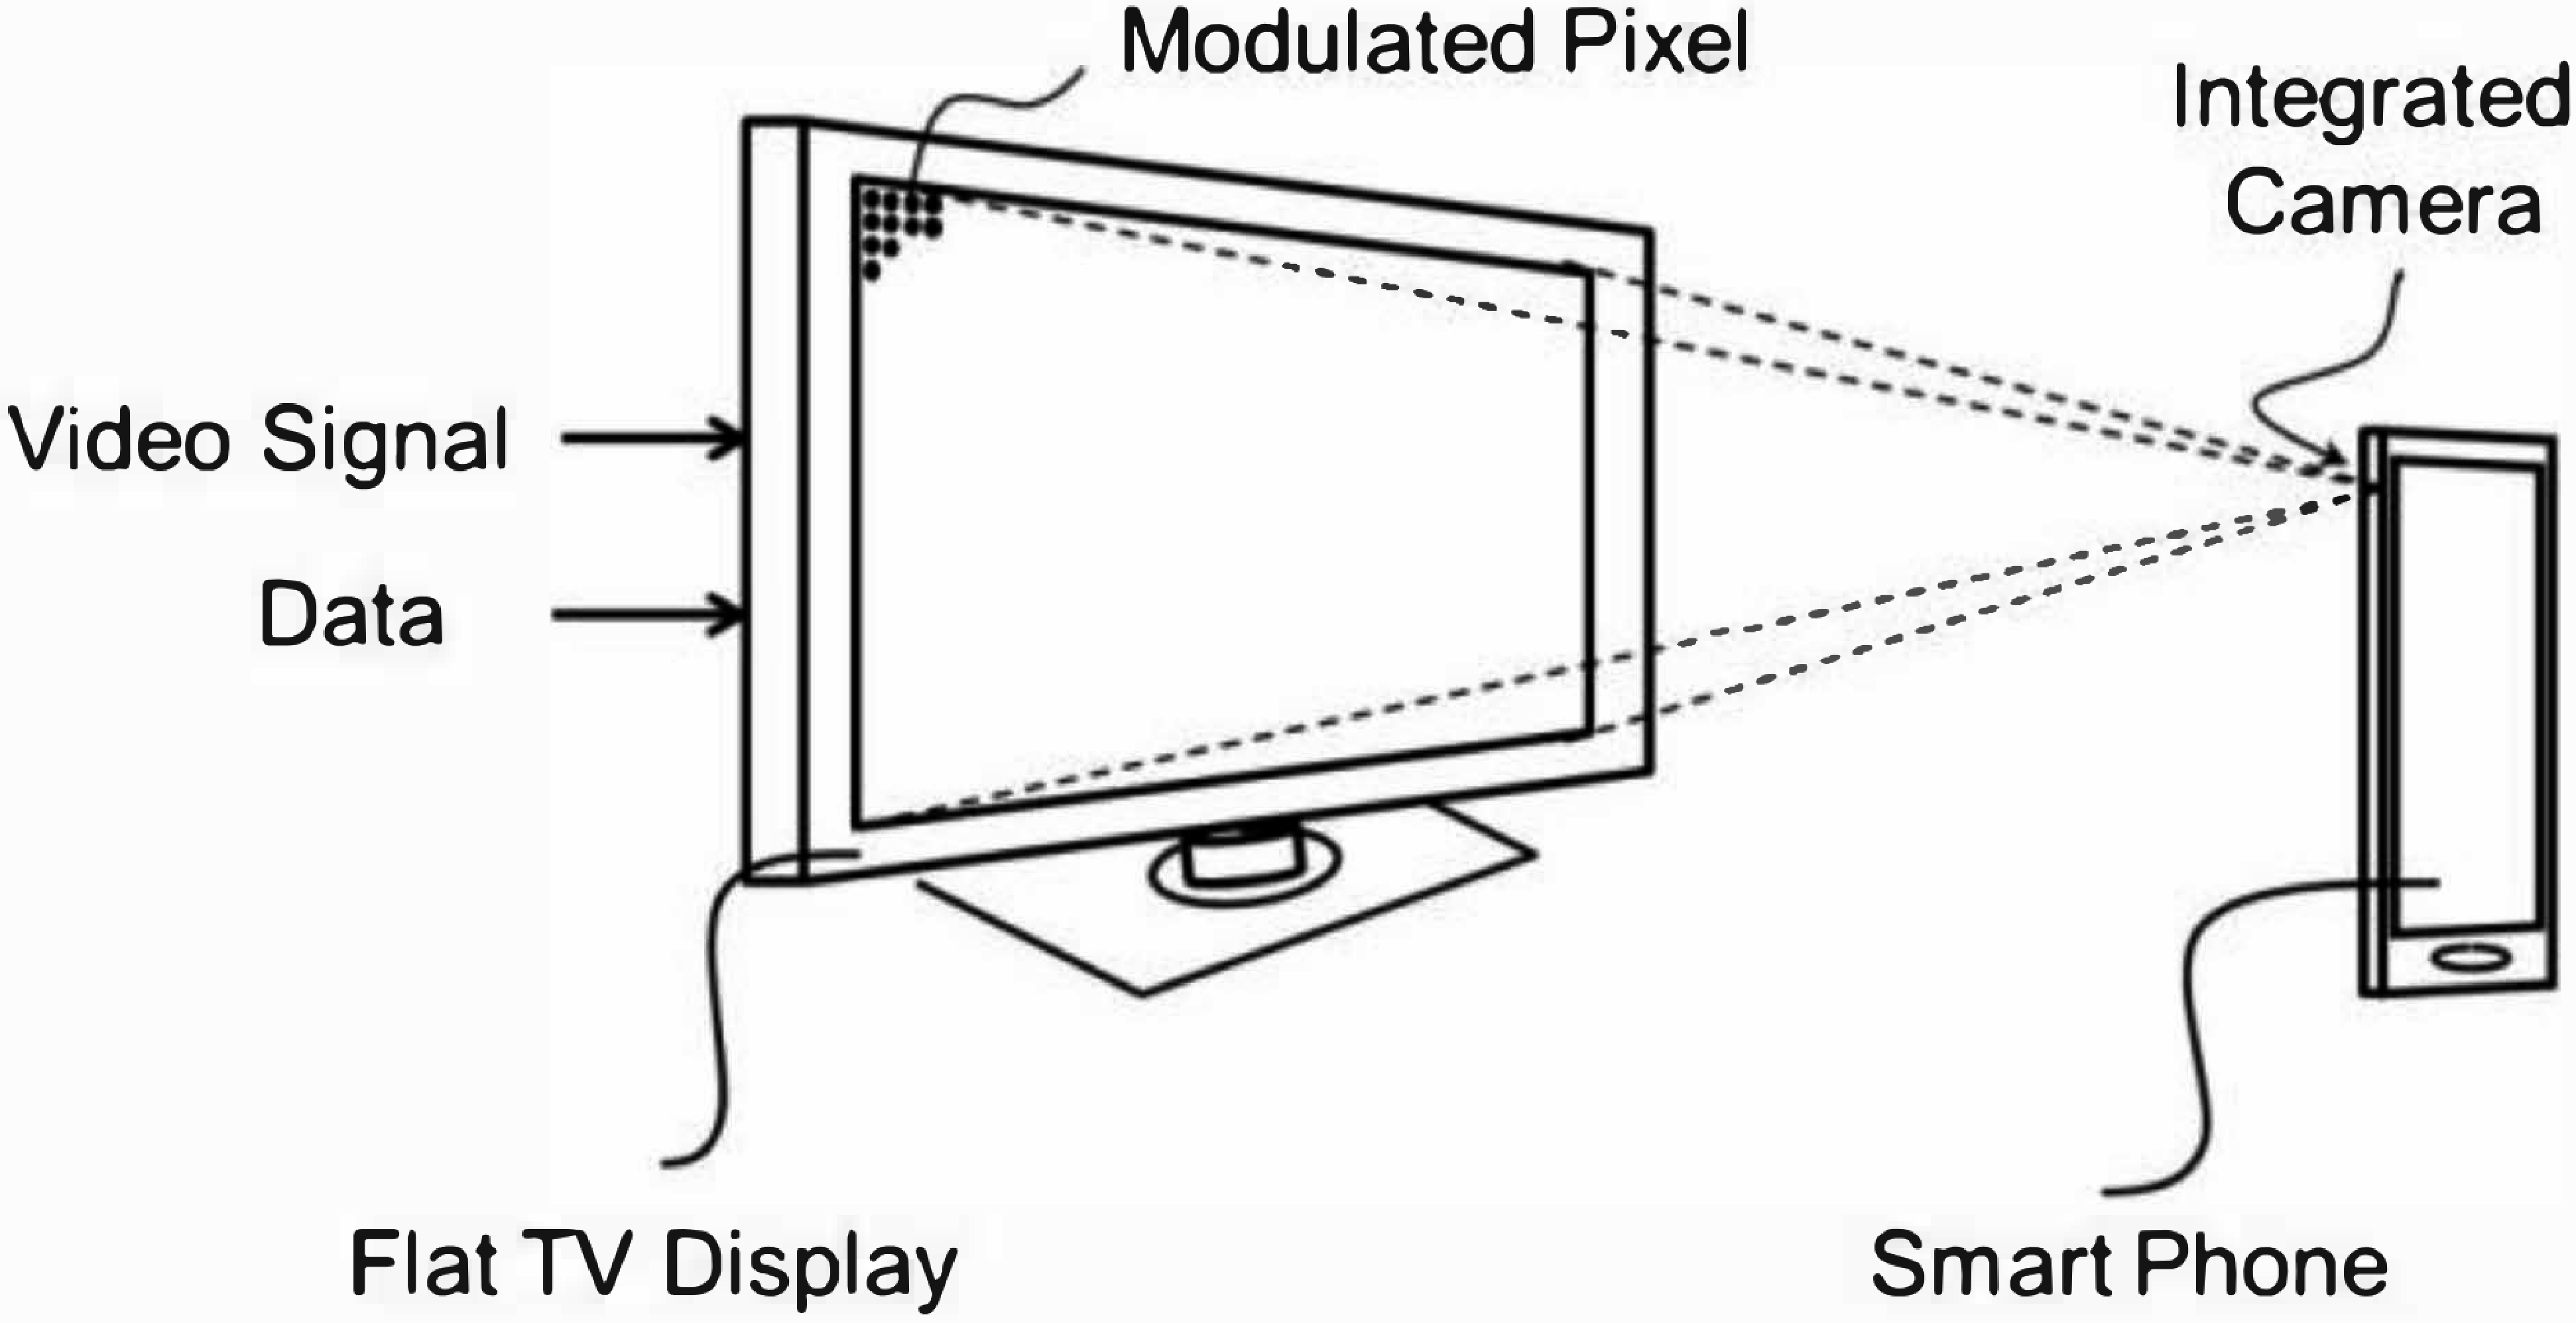
\includegraphics[keepaspectratio,width=0.8\textwidth]{images/2_DaViD/David1.pdf}
 \caption{Eine beispielhafte Implementierung des \gls{david}-Systems\cite{Kays201502}}
 \label{fig:David1}
\end{figure}


\section{Systemmodell} 
Das Display enthält eine große Anzahl von Pixel, die jeweils aus einer spezifischen Anordnung von Subpixel zur Darstellung des RGB-Farbraums bestehen. Jeder einzelne Frame des Videos wird durch eine Matrix von Subpixelwerten dargestellt. Das \gls{david}-System verwendet eine differentielle Modulationsmethode d.h. die Videoinformationen wird wiederholt, sodass Daten als ein Manchester-Code moduliert und zu den Videosignalkomponenten hinzugefügt werden. Durch eine zeitliche Synchronisation der Empfängerseite kann die \gls{isi} vermieden werden. Nach einer örtlichen Synchronisation mit dem modulierten Display, enthält der Empfänger ein Differenzbild. In Anschluss kann der Modulationsbereich, der durch die optische Projektion verzerrt wird, mit Verwendung der Verfahren in dieser Arbeit wiederherzustellen. Danach werden die überlagerten Datensequenz durch eine Reihe von Behandlungen, vom Videoinhalt getrennt. Abbildung \ref{fig:David2} zeigt die schematische Darstellung des \gls{david}-Systems. 
% Deshalb in zeitlicher oder örtlicher Richtung die Videoinhalt in paar Bildern werden gleich.



\vspace{18pt}

\begin{figure}[H]
	\centering 
	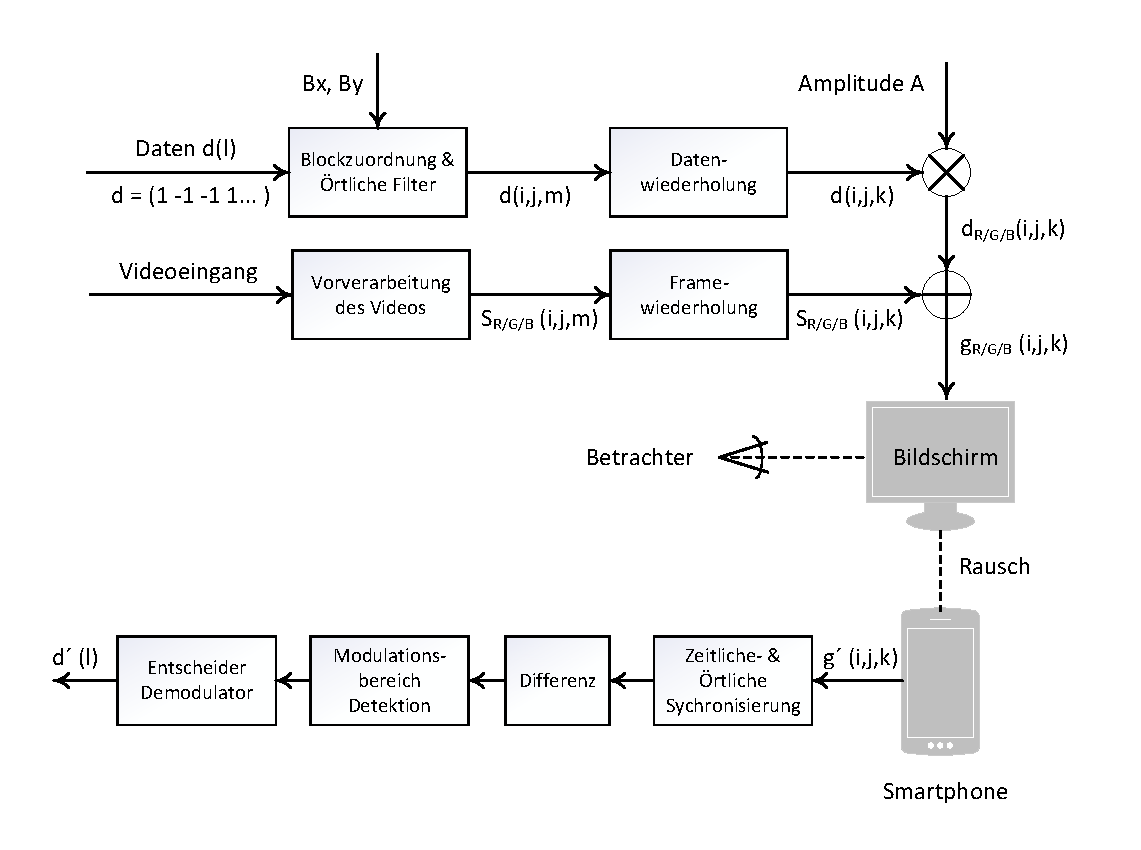
\includegraphics[keepaspectratio,width=1.0\textwidth]{images/2_DaViD/Systemmodell.pdf}
	\caption{Schematische Darstellung vom \gls{david}-System}
	\label{fig:David2}
\end{figure}


\subsection{Modulationsverfahren}

Ein Modulationsverfahren, welches die Videoqualität nicht beträchtlich reduziert, ist sehr kritisch für ein auf Videogeräte basierendes Datenübertragungssystem. Die möglichen Modulationsverfahren im \gls{david}-System sind:
\begin{itemize}
	\item Zeitlich-differentielle Modulation der Luminanz
	\item Zeitlich-differentielle Modulation der Chrominanz
	\item Örtlich-differentielle Modulation der Luminanz
	\item Örtlich-differentielle Modulation der Chrominanz
\end{itemize}

Zeitlich-differentielle Modulationsverfahren lassen eine Reihe von Frames paarweise den gleichen Luminanz- bzw. Chrominanz-Videoinhalt anzeigen. Dagegen haben die benachbarten Pixel bei örtliche-differentielle Modulation die gleichen Videoamplituden. In dieser Arbeit wird nur zeitlich-differentielle Modulation der Chrominanz verwendet, d.h. durch Subtrahieren dieser Frames entsteht ein Datensequenz Differenzbild, welches die beiden Verfahren in dieser Arbeit darauf basiert. %Abbildung \ref{fig:David3} zeigt ein Blockschaltbild einer typischen Senderimplementierung durch zeitlich-differentielle Modulation.

%\begin{figure}[htb]
%	\centering 
%	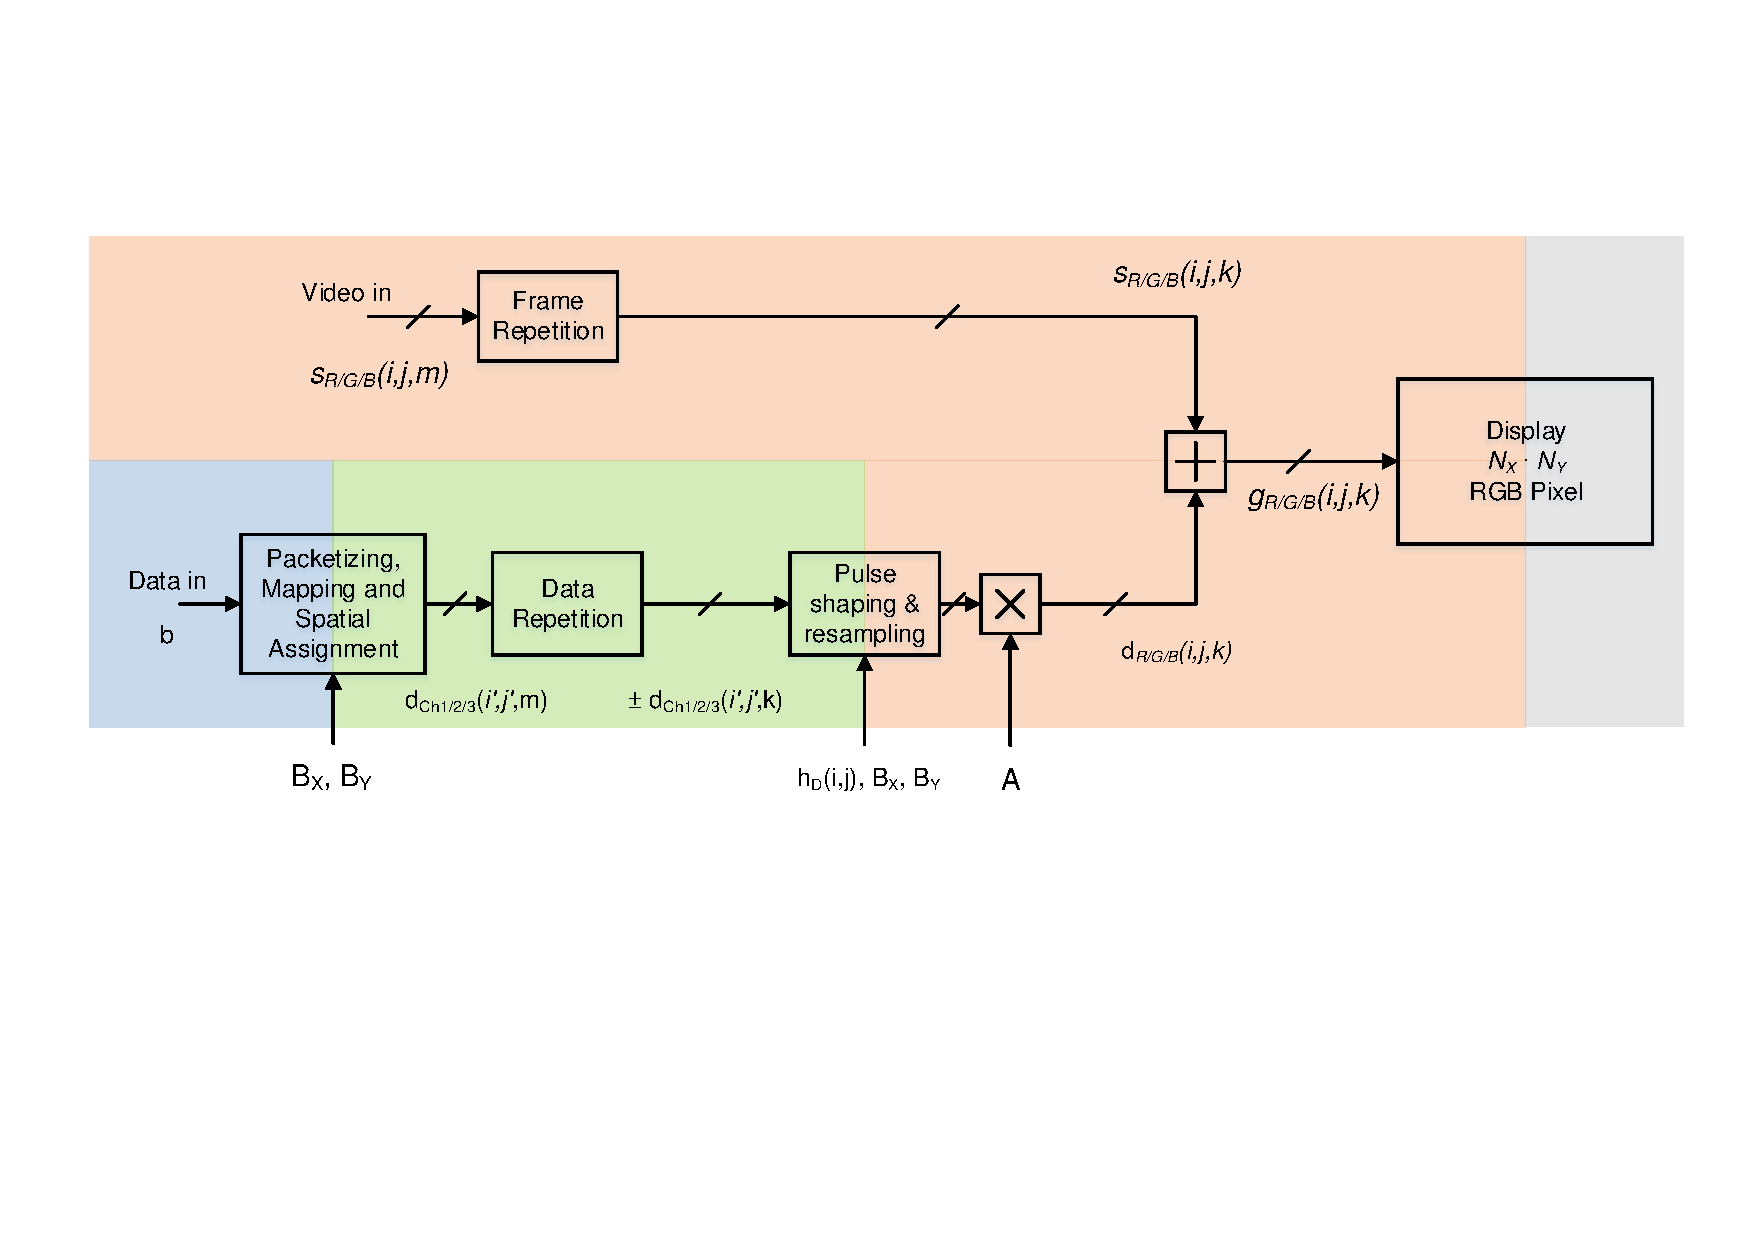
\includegraphics[keepaspectratio,width=0.8\textwidth]{images/2_DaViD/2.pdf}
%	\caption{Blockschaltbild der Signalverarbeitung in zeitlich-differentieller Modulation}
%	\label{fig:David3}
%\end{figure}

Es wird angenommen, eine Display enthält in horizontaler Richtung $N_x$ Pixel und in vertikaler Richtung $N_y$ Pixel. Ein Videoeingangssignal wird verarbeitet, um eine Anzeigeeingabe $s(i,j,k)$ auszusenden. Mit zeitlich-differentieller Modulation gleicht der Inhalt dieses Frames des darauf folgenden. Die Indizes i und j definieren die horizontale und vertikale Pixelposition auf dem Display, während k die Nummer des reproduzierten Frames ist. Indiz m symbolisiert den Zähler der Frames in einer Videosequenz. Der Amplitudenbereich des Videosignals sollte begrenzt sein um die Addition kleiner Datenamplituden A ohne Übersteuern zu ermöglichen.

\begin{equation}
\begin{split}
 s_{R/G/B}&(i,j,k+1) = s(i,j,k) \\
          &  for \ 0\le i <N_x, 0\le j<N_y,k=2m , m \in \mathbb{Z}\\
\end{split}
\end{equation}

%Vor der Datenübertragung muss der Datenstrom in Schichten der Länge L aufgeteilt werden. Indiz L bedeutet die Menge der Daten, die in einem Framepaar übertragen werden können. Ein direkter Ansatz ist eine direkte Zuordnung von Datenbits zu Pixeltripeln Zeile für Zeile.

%\begin{equation}
%\begin{split}
%  & d(l)\rightarrow d(i,j,m) \qquad d(l)\in \{-1,1\} \\
%  & 0\le l <L,L = N_x \cdot N_y \\
%  & i=l \bmod N_x \qquad j=\lfloor l/N_x \rfloor \\
%\end{split}
%\end{equation}

Die Modulationsamplitude A ist ein wichtiger Parameter für die Datenübertragung. Im Prinzip kann die Amplitude in verschieden Kanälen unabhängig gewählt werden um die Systemleistung zu optimieren. In dieser Arbeit werden alle Amplituden auf den gleichen Wert gesetzt.

\begin{equation}
 A_R=A_G=A_B=A        
\end{equation}

Das differentielle Modulationsverfahren ordnet jede Sequenz von $\left\{-A, A\right\}$ zu d = 0 bzw. $\left\{A, -A\right\}$ zu d = 1 zu. Modulierte Datensymbole und verarbeitete Videoamplituden werden addiert, um die Anzeigeeingabe $g(i,j,k)$ zu liefern:

\begin{equation}
\begin{split}
   g_{R/G/B}(i,j,k)  &= s_{R/G/B}(i,j,m) + A_{R/G/B} \cdot \left( 2 \cdot d(i,j,m) - 1 \right) \\
   g_{R/G/B}(i,j,k+1)&= s_{R/G/B}(i,j,m) - A_{R/G/B} \cdot \left( 2 \cdot d(i,j,m) - 1 \right) \\
\end{split}
\end{equation}

%Ein Beispiel einer modulierten Bildfolge ist in Abbildung \ref{fig:David4} gezeigt. Das Hinzufügen der modulierten Daten (hier mit A = 4) zu dem Videoeingang ergibt die Anzeigeamplituden in der rechten Spalte.
%\newpage

%\begin{figure}[htb]
%	\centering 
%	\includegraphics[keepaspectratio,width=0.6\textwidth]{images/2_DaViD/David4.jpg}
%	\caption{Ein Beispiel einer modulierten Bildfolge}
%	\label{fig:David4}
%\end{figure}

%Im Vergleich zu Luminanzteil Y ist die Anzeigequalität in der U und V Komponente signifikant besser, wenn Informationen in Chrominanz wiederholt und moduliert werden. Auf diese Weise wird die Gesamtleuchtdichte eines Pixel-Triples durch die Datenmodulation nicht beeinflusst. Die Umwandlungsmatrix (ITU-R BT.709) für \gls{HDTV} Display vom Standard $(R,G,B)$ zum Standard $(Y,U,V)$ ist folgende:

%\begin{equation}
%   T = \begin{pmatrix}
%   0,213 & 0,715 & 0,072 \\
%   -0,115& -0,385& 0,5	\\
%   0,5   & -0,454& -0,0458
%\end{pmatrix}  
%\end{equation}

%Das Videosignal $s(i,j,k)$ muss vor dem Anwenden der Modulation in Y-, U- und V-Komponenten umgewandelt werden. Die nachfolgende inverse Konvertierung erklärt das Display-Eingangssignal in Abbildung \ref{fig:David3}:

%\begin{equation}
%\begin{split}
%  \begin{pmatrix}
%  g_R(i,j,k) \\
%  g_G(i,j,k) \\
%  g_B(i,j,k) \\
%\end{pmatrix} &= T^{-1} \cdot \left( T \cdot \begin{pmatrix}
%  S_R(i,j,m) \\
%  S_G(i,j,m) \\
%  S_B(i,j,m) 
%  \end{pmatrix}  + \begin{pmatrix}
%  0 \\
%  A_U \cdot d(i,j,m) \\
%  A_V \cdot d(i,j,m) 
%  \end{pmatrix} \right) \\  
%  \begin{pmatrix}
%  g_R(i,j,k+1) \\
%  g_G(i,j,k+1) \\
%  g_B(i,j,k+1) \\
%\end{pmatrix} &= T^{-1} \cdot \left( T \cdot \begin{pmatrix}
%  S_R(i,j,m) \\
%  S_G(i,j,m) \\
%  S_B(i,j,m) 
%  \end{pmatrix}  - \begin{pmatrix}
%  0 \\
%  A_U \cdot d(i,j,m) \\
%  A_V \cdot d(i,j,m) 
%  \end{pmatrix} \right) \\ 
%\end{split}
%\end{equation}

%Diese Art der Modulation kann als eine Modulation des roten und des blauen Subpixels betrachtet werden, während der grüne Subpixel verwendet wird, um die Änderung der Luminanz des Pixel-Tripels zu kompensieren. Durch die Definition korreliert $A_U$ mit $A_B$ und $A_V$ mit $A_R$.
%
%\begin{equation}
%   \begin{pmatrix}
%   A_R \\
%   A_G \\
%   A_B
%  \end{pmatrix}  = T^{-1} \cdot \begin{pmatrix}
%   A_Y \\
%   A_U \\
%   A_V
%  \end{pmatrix}
%\end{equation}



\subsection{DatenBlock}

Ein einfaches und unkompliziertes Verfahren um die Anforderungen an die Kameraauflösung zu lockern, ist die Zuordnung jedes Datenbits zu einem Block von $B_X \times B_Y$ Pixel.
\begin{equation}
\begin{split}
  & d(l)\rightarrow d(x,y,k) \qquad 0\le l <L \\
  & L=\lfloor N_X/B_X \rfloor \cdot \lfloor N_Y/B_Y \rfloor \\
  & x=(l \cdot B_X) \bmod N_X +r_X, \ r_X =0...(B_X -1) \\
  & y=\lfloor l / \lfloor N_X/B_X \rfloor \rfloor \cdot B_Y +r_Y, \ r_Y =0...(B_Y -1) \\
\end{split}
\end{equation}

%Wenn die Anzahl der Pixel Pro Zeile bzw. Spalte kein Vielfaches von $B_X$ bzw. $B_Y$ ist, muss die Anzahl der Pixel Pro Zeile bzw Spalte, die für die Modulation in Gleichung $\left(2.8\right)$ verwendet werden, ersetzt werden durch:
%
%\begin{equation}
%\begin{split}
%  & N_X = \lfloor N_X/B_X \rfloor \cdot B_X\\ 
%  & N_Y = \lfloor N_Y/B_Y \rfloor \cdot B_Y\\ 
%\end{split}
%\end{equation}

In dieser Arbeit ist der Datenblock quadratisch.

\begin{equation}
   B_X = B_Y = B.
\end{equation}


\section{Anwendungsgebiete} 
%\label{sec:Anwendungsbereiche}

Die Datenübertragungsrate des \gls{david}-Systems beträgt voraussichtlich bis zu 100 Mbit/s. Es gehört zu einer Sichtlinienübertragung für kurze Strecken. Geeignete Abdeckungsbereiche hängen von der Größe des Displays und der Kameraoptik ab. Im Vergleich zu den letzten WLAN-Versionen des \gls{ieee} 802.11, erscheint die Leistung zunächst nicht attraktiv. Dieses spezielle Verfahren der Datenübertragung macht es jedoch zu einem Kandidaten für viele praktische Anwendungen. Außer den Hauptvorteilen von \gls{vlc} liegt der Vorteil auch in der Option zur Wiederverwendung der bestehenden Hardware, die zum Anzeigen des Videos eingebaut wurde. Ein geeigneter praktischer Anwendungsbereich des \gls{david}-Systems ist ein öffentlicher Ort, wie eine U-Bahn-Station, ein großes Stadion und Ähnliches. Angenommen in einer Situation, wo Passanten auf eine U-Bahn warten und ihre Software mit Hilfe von Digitalen Werbetafeln aktualisieren können, indem sie ihre Kamera auf die Werbung richten\cite{Kays201502}.

Durch Berücksichtigung der Eigenschaften des \gls{david}s, z.B. Synchronisation von Anwendungen und Datenübertragung, können viele attraktive Anwendungszenarien in Betracht gezogen werden. Drei Hauptszenarien sind: 

\begin{itemize}
  \item Indoor-individuelle Kommunikation: Kurzstreckenverbindungen basierend auf relativ kleinen (Tablet-Größe) Bildschirmen, Anwendungen wie z.B. die Übertragung von Hintergrundinformationen an Besucher im Museum oder Kiosk.
  \item Indoor-Multicast-Kommunikation: Streckenabstand ist länger als im ersten Fall auf relativ großem (40-100") Bildschirm, Anwendungen wie z.B. Herunterladen von Anwendungsdateien oder Mediendateien im Kiosk oder Restaurant.
  \item Freie Kommunikation: Riesige Bildschirme wie in Einkaufszentren oder Sport-Arenen. Anwendungen können denen des zweiten Szenarios ähneln.
\end{itemize}

Sobald die Dienste auf öffentlichen Bildschirmen implementiert werden, können Benutzer mit Hilfe eines modernen Smartphones mit einer geeigneten Kamera nach der Installation einer neuen App Innovation wahrnehmen.





















